\section{Symmetric Matrices}
%Lecture Sep 18

\begin{equation*}
S^n = \{A\in \Re^{n\times n} | A = A^T \}
\end{equation*}

Example: Hessian $[\nabla^2 F]_{ij} = \frac{\sigma}{\sigma x_i}\frac{\sigma}{\sigma x_j}F(x)$


Example: Quadratic Functions: $q: \Re^n \rightarrow \Re$

\begin{align*}
q(x) &= \sum^n_{i=1}\sum^n_{j=1}a_{ij}x_ix_j + \sum^n_{i=1}c_ix_i + d\\
&= x^TAx + c^Tx + d\\
&= \frac{1}{2}x^T(A + A^T)x + c^Tx + d\\
&= \frac{1}{2}
\begin{bmatrix}%
x^T& 1
\end{bmatrix}
\begin{bmatrix}%
A + A^T & C\\
C^T & 2d
\end{bmatrix}
\begin{bmatrix}%
x\\
1
\end{bmatrix}
\end{align*}


1) Let $F(x) = C^Tx = \sum^n_{i=1}c_ix_i$:

\begin{align*}
\frac{d}{dx_k}F(x) &= \frac{d}{dx_k}(\sum^n_{i=1}c_ix_i) = c_k\\
\nabla F(x) &= 
\begin{bmatrix}%
\frac{\sigma F(x)}{\sigma x_1}\\
...\\
\frac{\sigma F(x)}{\sigma x_n}
\end{bmatrix}=
\begin{bmatrix}%
c_1\\
...\\
c_n
\end{bmatrix} = C
\end{align*}

2) Let
\begin{align*}
F(x) &= x^TAx = \sum_i\sum_ja_{ij}x_ix_j\\
&= a_{11}x_1^2 + a_{12}x_1x_2 + ... + a_{21}x_2x_1 + ...\\
\frac{d}{dx_k}F(x) &= \frac{d}{dx_k}(a_{kk}k_k^2 + \sum_{l\neq k}k_lx_k(a_{kk}+a_{kl}))\\
&= (a_{kk} + a_{kk})x_k + \sum_{l\neq k}x_l(a_{lk} + a_{kl}) \\
&= \sum^n_{i=1}(a_{lk} + a_{kl})x_l\\
&= \sum^n_{i=1}([A]_{kl} + [A]_{lk})x_l
\end{align*}

\begin{align*}
\nabla F(x) &= (A + A^T)x\\
[\nabla^2F(x)]_{kj} &= \frac{d}{dx_j}(\frac{\partial}{\partial x_k}F(x))\\
&= [A]_{kj} + [A]_{jk}\\
\nabla^2F(x) &= (A + A^T)
\end{align*}

Because $q(x) = x^TAx + c^Tx + d$, take Taylor approximation of $q(x)$:

\begin{align*}
\tilde{q}(x) &= q(0) + \nabla q(0)^Tx + \frac{1}{2}x^T\nabla^2q(0)x\\
&= d + c^Tx + \frac{1}{2}x^T(A + A^T)x
\end{align*}

\subsection{Symmetric Matrices + Eigenvectors}

\begin{theorem}{4.18 \& 4.2 in textbook}
	For any matrix in $S^n = \{A\in \Re^{n\times n} | A = A^T \}$:
	
	1) All eigenvalues are purely real(so eigenvectors can be picked purely real)
	
	2) $GM(\lambda_i) = AM(\lambda_i)$: means always disgonalizable
	
	3) Eigenvectors of distinct eigenvalues are $\perp$.
	
	"Eigenspace"= $\xi_{x_i} = N(A - \lambda_iI)\perp \xi_{\lambda_i} = N(A - \lambda_jI)$
\end{theorem}

Implication: If we pick basis for each eigenspace $\lambda_i$ to be an orthogonal basis, because have "Fullset" of eigenvectors can always write:

"Spectral Decomposition":

\begin{align*}
A &= U\Lambda U^{-1}\\
&= U\Lambda U^{T}\\
&= 
\begin{bmatrix}%
u^{(1)} & u^{(2)} & ... & u^{(n)}\\
\end{bmatrix}
\begin{bmatrix}%
\lambda_1 & ... & ...\\
... & ... & ...\\
... & ... & \lambda_n
\end{bmatrix}
\begin{bmatrix}%
u^{(1)^T}\\
...\\
u^{(n)^T}
\end{bmatrix}\\
&= \sum^n_{i=1}\lambda_iU^{(i)}U^{(i)^T}
\end{align*}

\subsection{Variational Characterization of engenvalues of $\lambda_i$ where $A\in S^n$} 

Since all $\lambda_i \in \Re$ can order(largest-to-smallest):

\begin{equation*}
\lambda_{max}(A) = \lambda_1 \geq \lambda_2 \geq ... \geq \lambda_n =\lambda_{min}(A)
\end{equation*}

Ratio $\frac{x^TAx}{x^Tx}$ for $x\neq 0$ is a "Reyleigh quotient"

Thm(4.3): $\lambda_{min}(A) \leq \frac{x^TAx}{||x||^2}\leq \lambda_{max}(A), \forall x = 0$


\begin{proof}
	\begin{align*}
	x^TAx &= x^TU\Lambda U^Tx\\
	&= \bar{x}^T\Lambda\bar{x}\\
	&= \sum^n_{i=1}(\bar{x}_i)^2\lambda_i\\
	&\leq \sum^n_{i=1}(\bar{x}_i)^2\lambda_{max}(A)\\
	&= ||\bar{x}||^2\lambda_{max}(A)
	\end{align*}
	
	\begin{equation*}
	\lambda(A)_{min}||\bar{x}||^2 \leq x^TAx \leq ||\bar{x}||^2\lambda_{max}(A)
	\end{equation*}
	
	\begin{equation*}
	\lambda(A)_{min} \leq \frac{x^TAx}{||\bar{x}||^2} \leq \lambda_{max}(A)
	\end{equation*}
\end{proof}


\subsection{Positive (Semi)Definite matrices $\rightarrow$ "PD" or "PSD"}

\begin{definition}
	A symmetric matrix $A\in S^n$ is PD(alt PSD) if $x^TAx > 0$, $\forall x\in \Re^n$(alt $x^TAx\geq 0$)
\end{definition}

PSD: $S^n_{+} = \{A\in S^n | A\succeq 0\}$

PD: $S^n_{++} = \{A\in S^n | A\succ 0\}$

A symmetric matrix is PSD iff all its eigenvalues $\geq$ 0.

A symmetric matrix is PD iff all its eigenvalues $>$ 0.\\


(1) Assume $A\in S^n$ is PD $\rightarrow$ will show $\lambda_i > 0, \forall\,\,\, eigenvalues$.   

\begin{equation*}
x^TAx = x^TU\Lambda U^Tx = \bar{x}^T\Lambda\bar{x} = \sum^n_{i=1}\lambda_i(\bar{x}_i)^2 >0
\end{equation*}
Since A is PD and $x\neq 0$

To show this implies $\lambda_j > 0, \forall j\in [n]$, set:
$$\bar{x} = e_j = 
\left[
\begin{matrix}
0\\
0\\
...\\
1\\
0\\
0\\
...
\end{matrix}
\right]
$$
where only $j^m$ entry is 1.

\begin{equation*}
0 < U^{(i)^T} U\Lambda U^TU^{(1)} =e_j^T\Lambda e_j = \lambda_j
\end{equation*}



(2) Assume all eigenvalues positive $\rightarrow$ want to show A is PD:

\begin{equation*}
x^TAx =x^TU\Lambda U^Tx = \bar{x}^T\Lambda \bar{x} = \sum^n_{i=1}(\bar{x}_i)^2\lambda_i > 0
\end{equation*}

Last note:

$det(A) = \prod^n_{i=1}\lambda_i$

$det(A) = 0$ iff there is a $\lambda_i = 0$:

$\rightarrow$ PD matrices are invertible

$\rightarrow$ PSD matrices are invertible only if PD




\subsection{Ellipses} 

Consider the set:

\begin{equation*}
\xi = \{x\in \Re^n | (x - x^{(0)})^T P(x - x^{(0)}) \leq 1 \}
\end{equation*}

where P is PD.

Note argument is a quadratic function:

\begin{align*}
(x - x^{(0)})^TP^{-1}(x - x^{(0)}) &= x^TP^{-1}x - 2x^{(0)^T}P^{-1}x + x^{(0)^T}P^{-1}x^{(0)}\\
&= x^TAx + c^Tx + d
\end{align*}

Look at set $\xi$: $\rightarrow$ centered at $x = x^{(0)}$:

\begin{align*}
1 &\geq (x - x^{(0)})^TP^{-1}(x - x^{(0)})\\
&= \bar{x}^TP^{-1}\bar{x}\\
&= \bar{x}^T(U\Lambda U^T)^{-1}\bar{x}\\
&= \bar{x}^T(U^T)^{-1}\Lambda^{-1}U^{-1}\bar{x}\\
&= \bar{x}^TU\Lambda^{-1}U^T\bar{x}\\
&= xxx\\
&= \sum^n_{i=1}(\frac{\hat{x_i}}{\sqrt{\lambda_i}})^2\\
&= \sum^n_{i=1}(\hat{x}_i)^2\\
&= ||\hat{x}||^2
\end{align*}


\begin{figure}
	\centering
	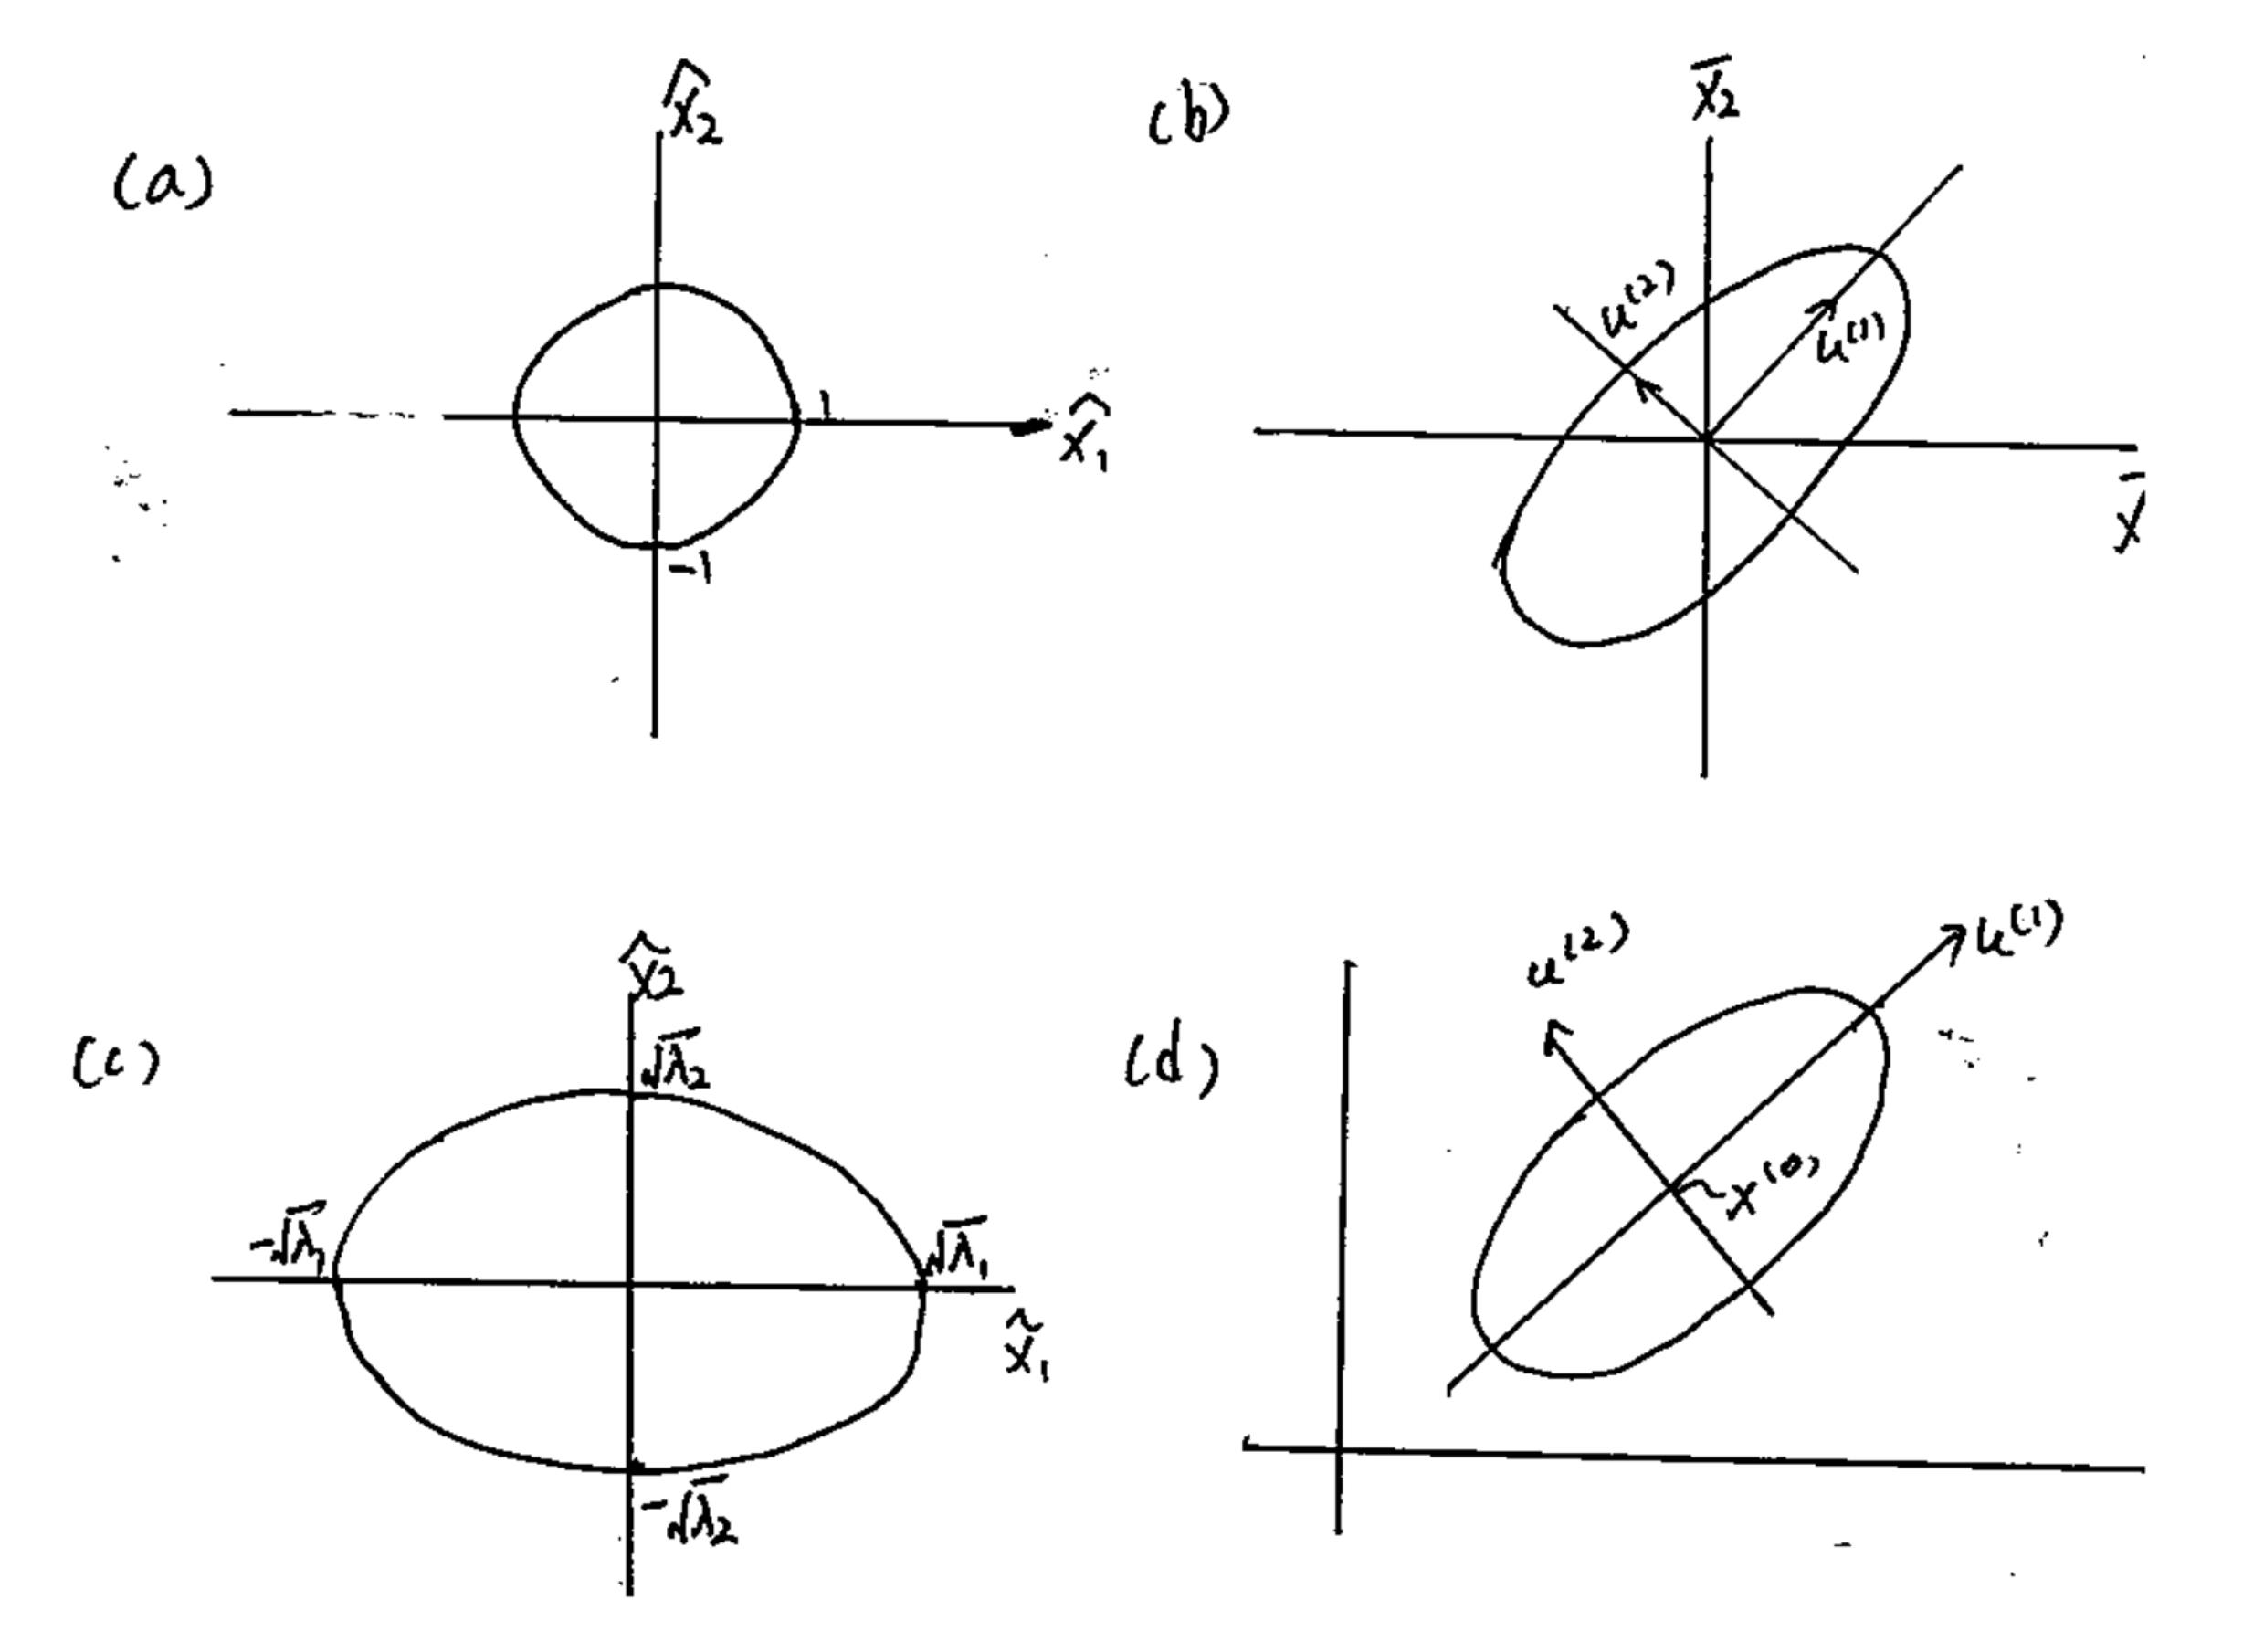
\includegraphics[width=2.1in,height=2.1in]{figures/ch03/figure2.jpg}
	%\caption{This is an inserted JPG graphic} 
	%\label{fig:graph} 
\end{figure}

Example: Sample covariance \& PSD matrices: 

Dataset $x^{(1)}, x^{(2)}, ..., x^{(m)}$ all $x^{(i)}\in \Re^n$\\

Sample mean: $\mu = \frac{1}{m}\sum^n_{i=1}x^{(i)}$

Sample covariance: $\sum = \frac{1}{m}\sum^m_{i=1}(x^{(i)}-\mu)(x^{(i)}-\mu)^T$

where $(x^{(i)}-\mu)(x^{(i)}-\mu)^T$ is the outer-product of centered data points.

m=3:

$$x^{(1)} =
\left[
\begin{matrix}
1\\
2
\end{matrix}
\right]x^{(2)} =
\left[
\begin{matrix}
4\\
4
\end{matrix}
\right]x^{(3)} =
\left[
\begin{matrix}
4\\
0
\end{matrix}
\right]\mu =
\left[
\begin{matrix}
3\\
2
\end{matrix}
\right]\tilde{x}^{(1)} =
\left[
\begin{matrix}
-2\\
0
\end{matrix}
\right]\tilde{x}^{(2)} =
\left[
\begin{matrix}
1\\
2
\end{matrix}
\right]\tilde{x}^{(3)} =
\left[
\begin{matrix}
1\\
-2
\end{matrix}
\right]
$$



$$\Sigma = 
\left[
\begin{matrix}
2&0\\
0&\frac{8}{3}
\end{matrix}
\right]
$$

\begin{equation*}
\xi_{\gamma} = \{(x - \mu)^T \Sigma^{-1}(x - \mu)\leq \gamma \}
\end{equation*}
($\gamma$ = 2)

Proving $\Sigma\geq 0$, consider sample variances

\begin{equation*}
S^{(1)} =w^Tx^{(1)} = <w, x^{(1)}>\,\,\, when \,\,\, ||w|| = 1
\end{equation*}

sample mean:

\begin{equation*}
\tilde{S} = \frac{1}{m}\sum^m_{i=1}s^{(i)} = \frac{1}{m}\sum^m_{i=1}w^Tx^{(1)} = w^T\mu
\end{equation*}



sample variance: 

\begin{align*}
\sigma^2 &= \frac{1}{m}\sum^m_{i=1}(s^{(i)} - w^T\mu)^2 \\
&= \frac{1}{m}\sum^m_{i=1}(w^T(x^{(i)} -\mu))^2\\
&=\frac{1}{m}\sum^m_{i=1}w^T(x^{(i)}-\mu)(x^{(i)}-\mu)^Tw\\
&= w^T[\frac{1}{m}\sum^m_{i=1}(x^{(i)}-\mu)x^{(i)}-\mu)^T]w\\
&= w^T\sum w
\end{align*}



\subsection{Square-root matrix}

For any PSD,

\begin{align*}
A &= U\Lambda U^{-1} \\
&=U\Lambda^{\frac{1}{2}}\Lambda^{\frac{1}{2}}U^{T}\,\, where \,\,\, \Lambda^{\frac{1}{2}}
\begin{bmatrix}%
\sqrt{\lambda_1}&...&...\\
...&...&...\\
...&...&\sqrt{\lambda_n}
\end{bmatrix}\\
&= U\Lambda^{\frac{1}{2}}U^TU\Lambda^{\frac{1}{2}}U^T
\end{align*}

where $A^{\frac{1}{2}} = U\Lambda^{\frac{1}{2}}U^T$ $\rightarrow$ "sq-root" matrix. 
